\section{Case Study}


\begin{figure}[tb]
	\centering
	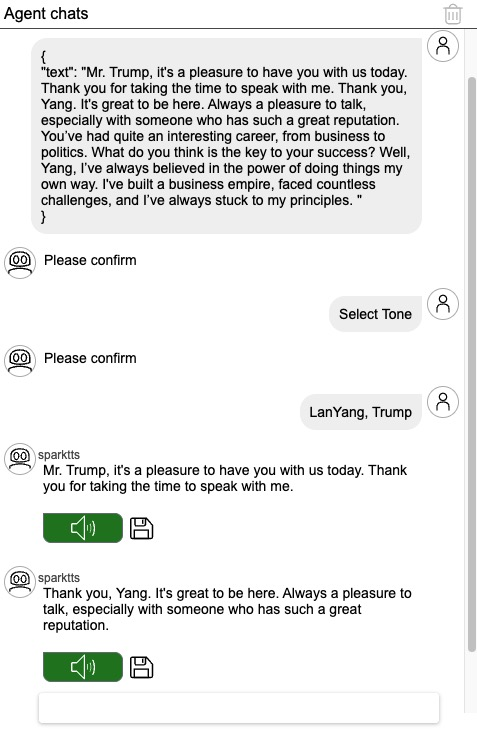
\includegraphics[scale=0.4]{imgs/generation.png}
	\caption{Screenshot of the user interface after auto-deployment.}
	\label{fig:gen}
\end{figure}

%\footnote{Model download time is excluded, as it depends on network speed.}

\begin{figure}[tb]
    \centering
    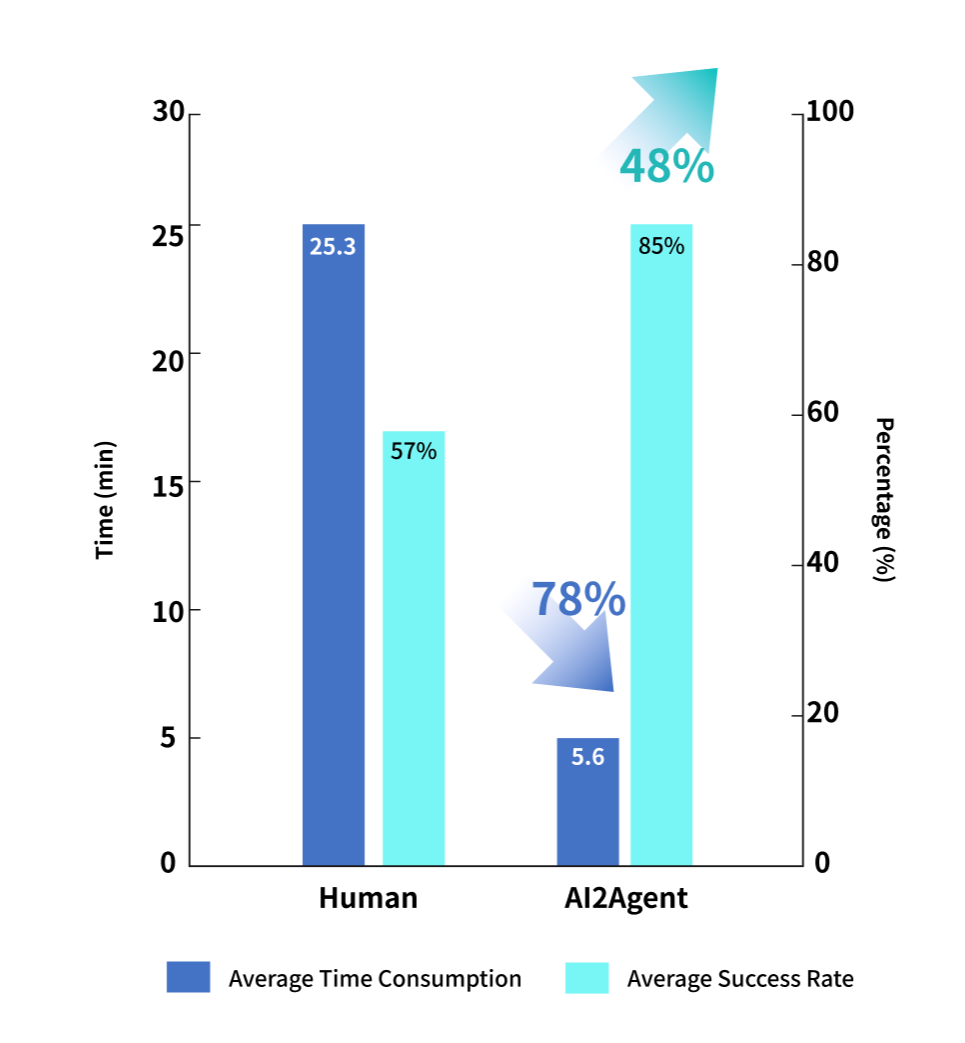
\includegraphics[scale=0.4]{imgs/score.png}
    \caption{
        Comparison of manual vs. AI2Agent deployment:  
        (1) \textbf{Time Consumption}: AI2Agent reduces deployment time by 78\%.  
        (2) \textbf{Success Rate}: AI2Agent improves success rate by 48\%.  
    }
    \label{fig:score}
\end{figure}

To evaluate the effectiveness of AI2Agent in automating AI project deployments, we conducted a comprehensive study across 30 AI applications, including text-to-speech (TTS), text-to-image generation, and image editing. Figure~\ref{fig:gen} showcases a sample user interface from a successfully deployed project. This section further details details our deployment environment, evaluation setup, and a demo case of Spark-TTS.

\subsection{Deployment Environment}
We conducted all experiments using our self-developed \textbf{AI2Apps IDE~\cite{ai2apps}}, which is based on a web container framework. AI2Apps IDE is available in both web-based and locally deployed versions. To ensure security and full control over execution, all cases in this study were conducted using the locally deployed version. This approach guarantees that AI project installations and configurations are fully automated within a sandboxed environment, mitigating potential security risks associated with external dependencies and permissions.

\subsection{Evaluation Setup}
We assessed AI2Agent's performance across 30 AI applications spanning multiple domains, including text-to-speech (TTS), text-to-image generation, and image editing. To establish a fair comparison, we recruited participants with deep learning experience and provided them with guideline documents for manual deployment. Each participant independently attempted to deploy the applications without automation assistance.

To quantify AI2Agent’s effectiveness, we evaluated two key metrics:
\textbf{Deployment Time Reduction}: The average time required for installation and configuration, excluding model download time, as it is influenced by network speed.
\textbf{Success Rate Improvement}: The percentage of successful deployments completed without additional troubleshooting.


As shown in Figure~\ref{fig:score}, AI2Agent achieved a \textbf{78\%} reduction in average deployment time and a \textbf{48\%} increase in overall success rate, demonstrating its ability to streamline and enhance AI deployment efficiency.

\subsection{Demonstration: Deploying Spark-TTS}
To showcase AI2Agent’s automation capabilities, we present a case study on deploying \textbf{Spark-TTS}, a powerful text-to-speech (TTS) system. AI2Agent autonomously manages the entire setup process, including dependency management, model configuration, and environment preparation, ensuring a streamlined and error-free deployment. As illustrated in the user interface shown in Figure~\ref{fig:gen} and video\href{https://github.com/Avdpro/ai2apps}, AI2Agent significantly reduces manual effort while maintaining a high success rate. The final speech output demonstrates excellent pronunciation accuracy, fluency, and overall quality, further validating the effectiveness of the framework.